\usepackage[spanish]{babel}
%Para uso de palabras acentuadas
\usepackage[utf8]{inputenc}

\documentclass[a4paper]{article}
\usepackage[utf8]{inputenc}
\usepackage[spanish, es-tabla, es-noshorthands]{babel}
\usepackage[table,xcdraw]{xcolor}
\usepackage[a4paper, footnotesep = 1cm, width=20cm, top=2.5cm, height=25cm, textwidth=18cm, textheight=25cm]{geometry}
%\geometry{showframe}

\usepackage{tikz}
\usepackage{amsmath}
\usepackage{amsfonts}
\usepackage{amssymb}
\usepackage{float}
\usepackage{graphicx}
\usepackage{caption}
\usepackage{subcaption}
\usepackage{multicol}
\usepackage{multirow}
\setlength{\doublerulesep}{\arrayrulewidth}
\usepackage{booktabs}

\usepackage{hyperref}
\hypersetup{
    colorlinks=true,
    linkcolor=blue,
    filecolor=magenta,      
    urlcolor=blue,
    citecolor=blue,    
}

\newcommand{\quotes}[1]{``#1''}
\usepackage{array}
\newcolumntype{C}[1]{>{\centering\let\newline\\\arraybackslash\hspace{0pt}}m{#1}}
\usepackage[american]{circuitikz}
\usetikzlibrary{calc}
\usepackage{fancyhdr}
\usepackage{units} 

\graphicspath{{../Ejercicio-1/}{../Ejercicio-2/}{../Ejercicio-3/}{../Ejercicio-4/}}

\pagestyle{fancy}
\fancyhf{}
\lhead{22.01 Teoría de Circuitos}
\rhead{Mechoulam, Lambertucci, Rodriguez Turco, Londero, Galdeman}
\rfoot{\centering \thepage}

\usepackage{float}
\usepackage{graphicx}

\usepackage[american voltage]{circuitikz}

\usepackage{amsmath}

\usepackage{xcolor}

\usepackage{caption}
\usepackage{subcaption}

\begin{document}

\section{Circuitos integradores y derivadores}
\subsection{Introducción}
Los circuitos implementados con amplificadores operacionales permiten la implementación de diferentes configuraciones que resuelven problemas matemáticos. Con el diseño adecuado pueden usarse para resolver sistemas de ecuaciones diferenciales.
En este caso estudiaremos 2 bloques fundamentales. El circuito integrador y el derivador. Se analizaran sus características más relevantes así como también sus límites de uso y como extenderlos para aprovecharlos al máximo.

\begin{figure}[hbt!]
	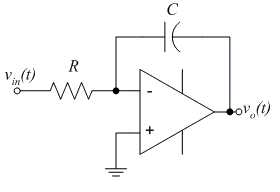
\includegraphics[scale=1]{Ejercicio4/integrador.png}
	\caption{Circuito integrador} 
	
	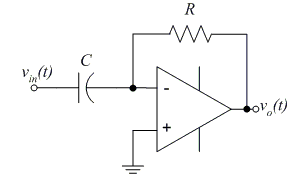
\includegraphics{Ejercicio4/derivador}
	\caption{Circuito Derivador} 
	
\end{figure}

\subsection{Análisis previo del \textbf{LM833N}}
El amplificador a utilizar es el \textbf{LM833N} de STMicroelectronics. El mismo es un operacional de bajo ruido diseñado para aplicaciones relacionadas al manejo de audio.
En su hoja de datos podemos ver que posee un alto nivel Slew Rate de hasta 7 $\frac{V}{s}$, un GBP de 15MHz y una ganancia de tensión 
a lazo abierto típica de unos 110 dB. Notemos que también se indica que la ganancia mínima es de unos 90 dB. 


 \subsubsection{Cálculo de $A_{vol}$}
Para poder realizar los cálculos de transferencia y establecer sus correspondientes transferencias de teóricas primero debemos conocer $A_{vol}$ medido en veces. Para esto basta con tomar el valor de ganancia de tensión típica a veces.
$$A_{vol} = 10^{\frac{110}{20}}$$
$$A_{vol} \approx 316.227,77$$

\subsubsection{Cálculo de  la $f_p$, polo dominante}

Dado el \textbf{GBP} de 15MHz podemos fácilmente calcular la frecuencia de corte a lazo abierto

$$ f_p = \frac{15MHz}{A_{vol}} $$
$$ f_p \approx 47.44Hz$$

\section{Ganancia bajo diferentes condiciones de $A_{vol}$}
En esta sección analizaremos las características de la ganancia de tensión brindad por ambos circuitos bajo diferentes condiciones.

\subsection{$A_{vol}$ infinito}
En un circuito con amplificadores operacionales es deseable utilizar dispositivos con $A_{vol}$(ganancia a lazo abierto) lo más alto posible para que los modelos teóricos se aproximen a su implementación física.

Ambos circuitos adoptan la configuración de un circuito inversor y sus transferencias pueden ser descritas mediante
$$H(s)_{inv} = \frac{-\frac{Z_{Feed}}{Z_{in}}}
{1+\frac{1+\frac{Z_{Feed}}{Z_{in}}}{A_{vol}}} $$
La cual representa la función transferencia de un amplificador operacional no ideal.
Si consideramos $A_{vol}$ infinito obtenemos la transferencia para el inversor ideal:
$$H(s)_{inv} = \frac{-\frac{Z_{Feed}}{Z_{in}}}
				{1+\underbrace{\frac{1+\frac{Z_{Feed}}{Z_{in}}}{A_{vol}}}_{\text{\shortstack{$A_{vol}\rightarrow \infty$ \\ $\rightarrow 0$}}}}$$

$$H(s)_{ideal} =  -\frac{Z_{Feed}}{Z_{in}}$$

Entonces para el circuito integrador obtenemos:
$$H(s)_{\int_{}{}} = \frac{-1}{sCR} $$

Podemos corroborar que la acción de este circuito es integrar la señal de entrada al realizar la transformada inversa de Laplace
$$v_{out}(t) = \mathcal{L}^{-1}[X(s)H(s)_{\int_{}{}}]$$
$$v_{out}(t) = \mathcal{L}^{-1}[X(s)\cdot \frac{-1}{sCR}]$$
$$v_{out}(t)= \frac{-1}{CR} \cdot \int_{0}^{t}v_t dt$$            
\\
Por otro lado tenemos el circuito derivador:
$$H(s)_{\frac{d}{dt}}=-sCR$$
Análogamente aplicamos la anti-transformada de Laplace:

$$v_{out}(t) = \mathcal{L}^{-1}[X(s)H(s)_{\frac{d}{dt}}]$$

$$v_{out}(t) = \mathcal{L}^{-1}[X(s)\cdot (-sCR)]$$

$$v_{out}(t)= -CR \frac{d}{dt}v_t(t)$$       

Si bien, estos circuitos tienen la capacidad de realizar las operaciones antes mencionadas, en los párrafos siguientes estudiaremos su comportamiento y bajo que condiciones funcionan.

\subsubsection{Diagramas de Bode con $A_{vol}$ ideal}
\begin{figure}[H]
	\centering
	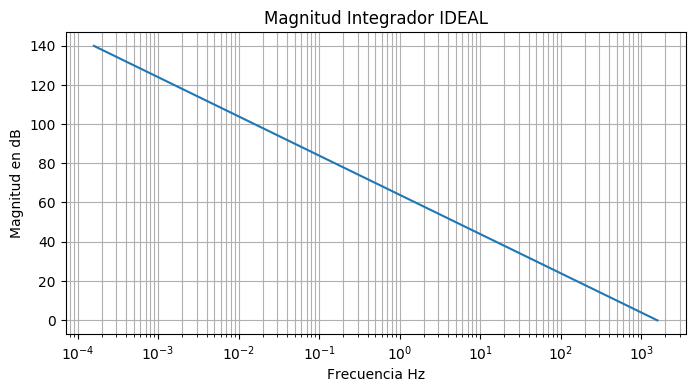
\includegraphics[width=\textwidth]{Ejercicio4/BODE-IDEAL-MAGNITUD-INTEGRADOR.png}
	\caption{Ganancia Ideal Circuito Integrador}
\end{figure}

Observamos que el integrador ideal tiene una muy alta ganancia a bajas frecuencias y muy baja cuando se acerca a los $10KHz$ lo cual limita su rango de operación.

\begin{figure}[H]
	\centering
	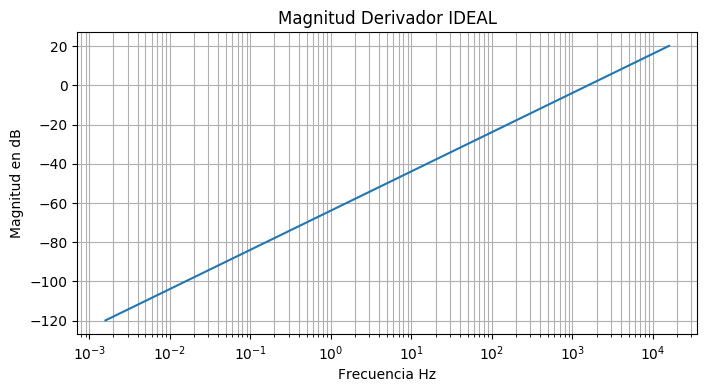
\includegraphics[width=\textwidth]{Ejercicio4/BODE-IDEAL-MAGNITUD-DERIVADOR.png}
	\caption{Ganancia Ideal Circuito Derivador}
\end{figure}
De modo contrario el derivador exhibe sus capacidades a altas frecuencias
\\*
En cuanto a la fase en ambos casos podemos observar como ver cómo las operaciones de integración y diferenciación introducen un desfase de $\pm90^{\circ}$ de la señal original según el caso. 
\begin{figure}[H]
	\centering
	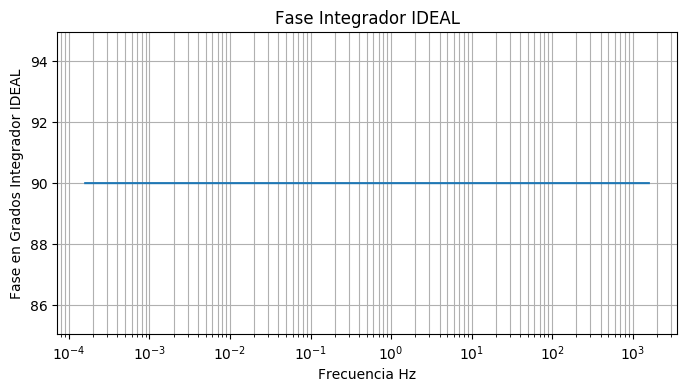
\includegraphics[width=\textwidth]{Ejercicio4/BODE-IDEAL-FASE-INTEGRADOR.png}
	\caption{Fase Ideal Circuito Integrador}
\end{figure}

\begin{figure}[H]
	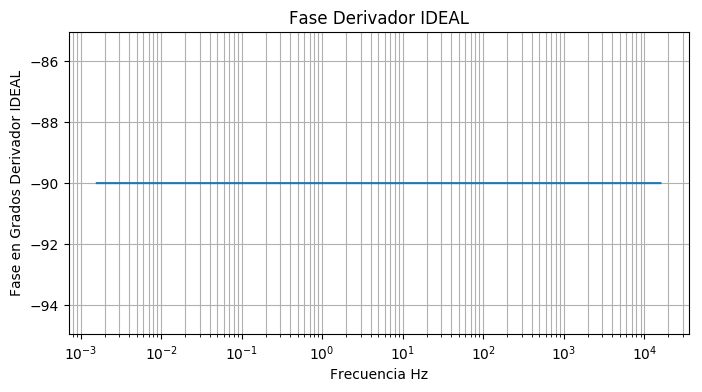
\includegraphics[width=\textwidth]{Ejercicio4/BODE-IDEAL-FASE-DERIVADOR.png}
	\caption{Fase Ideal Circuito Derivador}
\end{figure}

\subsection{$A_{vol}$ finito}
La ganancia a lazo abierto nunca es infinita en los amplificadores operacionales aunque por cuestiones de simplicidad podemos tratarlo como así fuese. En la introducción calculamos el $A_{vol}$ del \textbf{LM833} a partir de los datos brindados por el fabricante en la hoja de datos y encontramos que este valor se encuentra aproximadamente en $316.227,77$.
Ahora podemos volver a mirar a la función transferencia del inversor no ideal presentada al comienzo.
$$H(s)_{inv} = \frac{-\frac{Z_{Feed}}{Z_{in}}}
{1+\frac{1+\frac{Z_{Feed}}{Z_{in}}}{A_{vol}}} $$


\subsubsection{Diagramas de Bode con $A_{vol}$ finito}
Considerando $A_{vol}$ finito obtenemos las siguientes transferencias modificadas.

Para el \textbf{integrador} tenemos que $Z_{in}=R$, $Z_{feed}=\frac{1}{sCR}$
$$H(s)=\frac{-A_{vol}}{sCR(A_{vol}+1)+1}$$

Por otro lado para \textbf{derivador} las impendancias de entrada y feedback seran $Z_{in} = \frac{1}{sC}$ y $Z_{feed}  = R$
$$H(s) = - \frac{A_{vol} C R s \omega_p}{A_{vol} \omega_p + \left(s + \omega_p\right) \left(C R s + 1\right)}$$
Y se obtienen las siguientes diagramas de Bode Teóricos 

\begin{figure}[H]
	\centering
	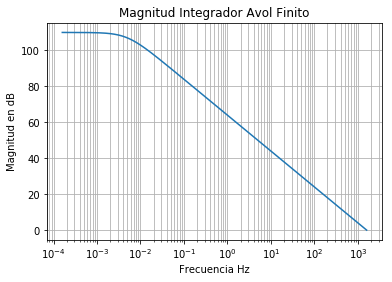
\includegraphics[width=\textwidth]{Ejercicio4/BODE-AVOL-FINITO-MAGNITUD-INTEGRADOR}
	\caption{Ganancia con $A_{vol}$ finito Circuito Integrador}
\end{figure}
El tipo de integrador analizado aquí comienza a integrar aproximadamente para señales de 5$mHz$ en adelante. Sin embargo su alta ganancia hace que una señal de 150 $mV$ a 1$mHz$ sature la salida del opamp. Veremos más adelante como esta característica afecta significativamente el desempeño del este circuito.
\begin{figure}[H]
	\centering
	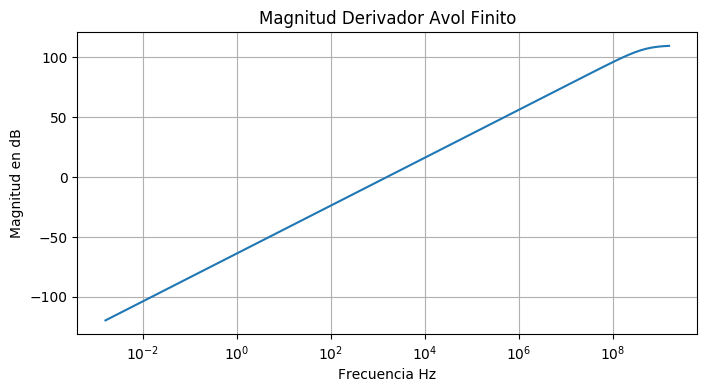
\includegraphics[width=\textwidth]{Ejercicio4/BODE-AVOL-FINITO-MAGNITUD-DERIVADOR}
	\caption{Ganancia con $A_{vol}$ finito Circuito Integrador}
\end{figure}

En el caso del derivador ocurre lo contrario, es necesario alcanzar frecuencias en el orden de los $100KHz$ para poder ver una señal sin tanta atenuación. Pero tampoco sera posible y mucho más allá dado que la ganancia brindada rápidamente saturara al operacional lo cual nuevamente limita el rango de operación del circuito. 

\begin{figure}[H]
	\centering
	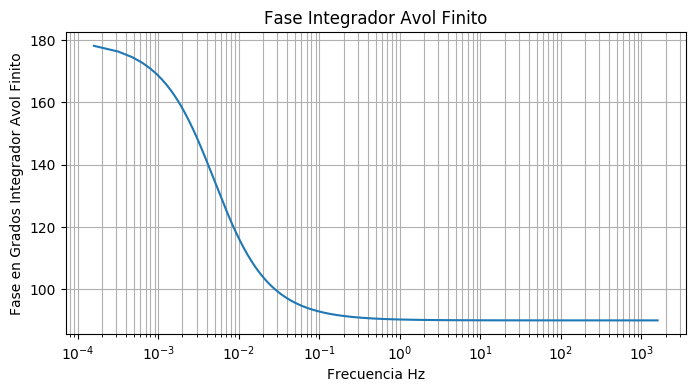
\includegraphics[width=\textwidth]{Ejercicio4/BODE-AVOL-FINITO-FASE-INTEGRADOR}
	\caption{Fase con $A_{vol}$ finito Circuito Integrador}
\end{figure}

\begin{figure}[H]
	\centering
	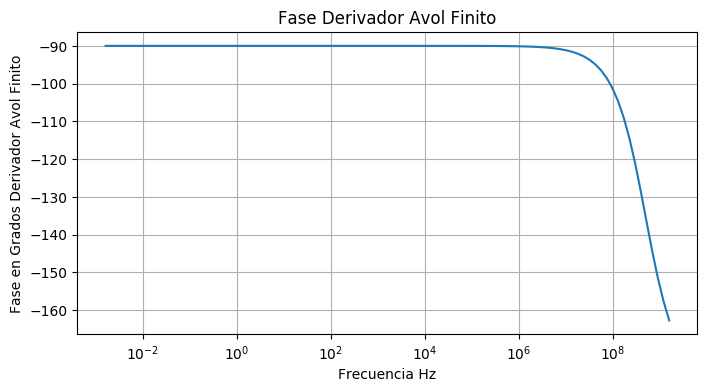
\includegraphics[width=\textwidth]{Ejercicio4/BODE-AVOL-FINITO-FASE-DERIVADOR}
	\caption{Fase con $A_{vol}$ finito Circuito Integrador}
\end{figure}

\subsection{Análisis con Polo Dominante}
Con la finalidad de obtener resultados más predecible y garantizar la estabilidad del opamp, los fabricantes añaden el llamado \textbf{polo dominante}.
Por lo tanto ahora consideraremos:
$$A(s)=\frac{A_{vol}}{1+\frac{s}{\omega_p}}$$

Reemplazando en las expresiones de la sección anterior obtenemos
$$H(s)_{\int}=- \frac{\omega_p A_{vol}}{\left(s + \omega_p\right) \left(s c r{\left (\frac{s + \omega_p A_{vol} + \omega_p}{s + \omega_p} \right )} + 1\right)}$$


\begin{figure}[H]
	\centering
	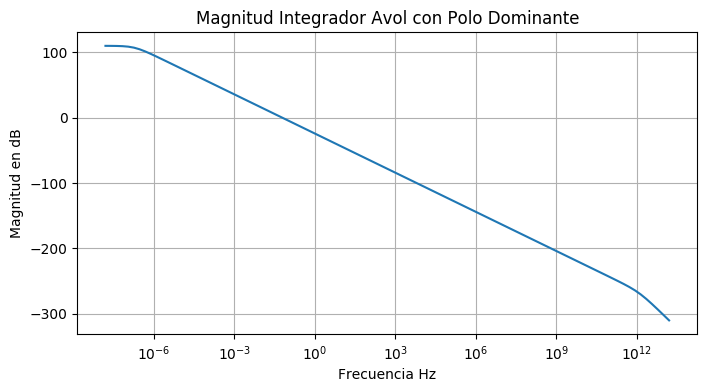
\includegraphics[width=\textwidth]{Ejercicio4/BODE-AVOLW-MAGNITUD-INTEGRADO}
	\caption{Ganancia con $A_{vol}(s)$ Polo Dominante Circuito Integrador}
\end{figure}
Notamos que no hay grandes diferencias en cuanto a su comportamiento al añadir el polo dominante. Sin embargo, se observa que para frecuencias de más de $1GHz$ comienzan a afectar los demás polos presentes en el opamps

\begin{figure}[H]
	\centering
	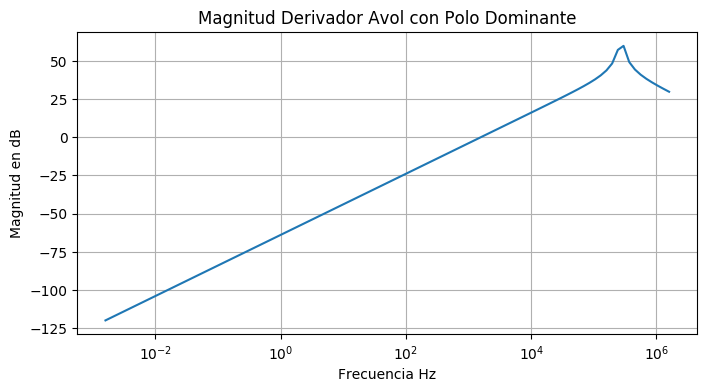
\includegraphics[width=\textwidth]{Ejercicio4/BODE-AVOLW-MAGNITUD-DERIVADOR}
	\caption{Ganancia con $A_{vol}(s)$ Polo Dominante Circuito Derivador}
\end{figure}
El caso del derivador en más interesante ya que al contrario de la sección anterior, aquí se nos presentan de manera evidente las limitaciones practicas de este circuito. 
En el rango de frecuencias bajas esta configuración presenta una atenuación significante por lo que la amplitud de entrada sera un factor critico. 


\begin{figure}[H]
	\centering
	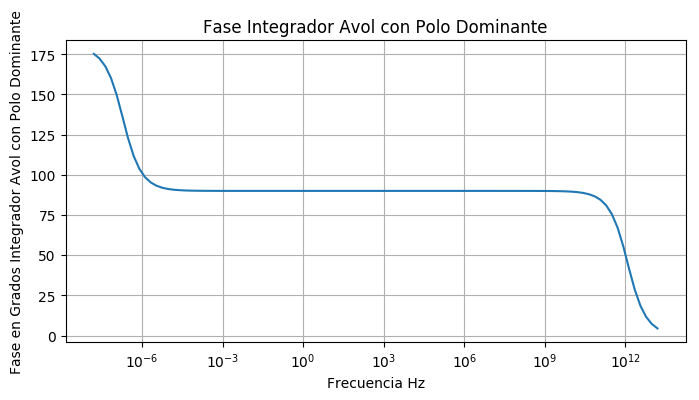
\includegraphics[width=\textwidth]{Ejercicio4/BODE-AVOLW-FASE-INTEGRADO}
	\caption{Fase con $A_{vol}(s)$ Polo Dominante Circuito Integrador}
\end{figure}


\begin{figure}[H]
	\centering
	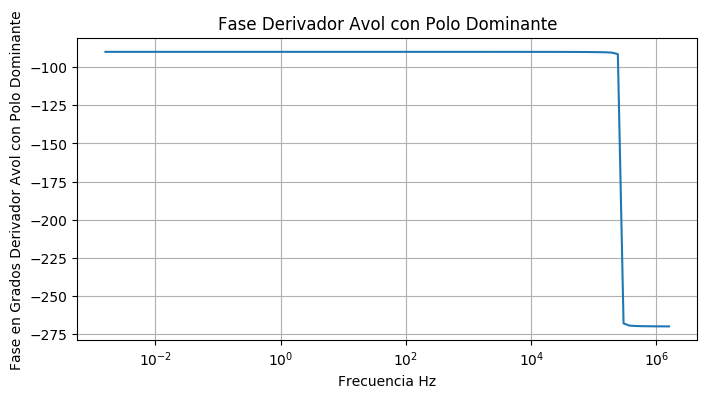
\includegraphics[width=\textwidth]{Ejercicio4/BODE-AVOLW-FASE-DERIVADOR}
	\caption{Fase con $A_{vol}(s)$ Polo Dominante Circuito Derivador}
\end{figure}

\section{Respuesta en frecuencia}
\subsubsection{Integrador NO Compensado}
El circuito integrador no compensado presenta una muy alta ganancia a bajas frecuencia lo cual produce saturación a la salida. Se utilizaron señales del orden de los 150 $mV$ para poder realizar las mediciones a bajas frecuencias.
%Bode integrador 
\begin{figure}[H]
	\centering
	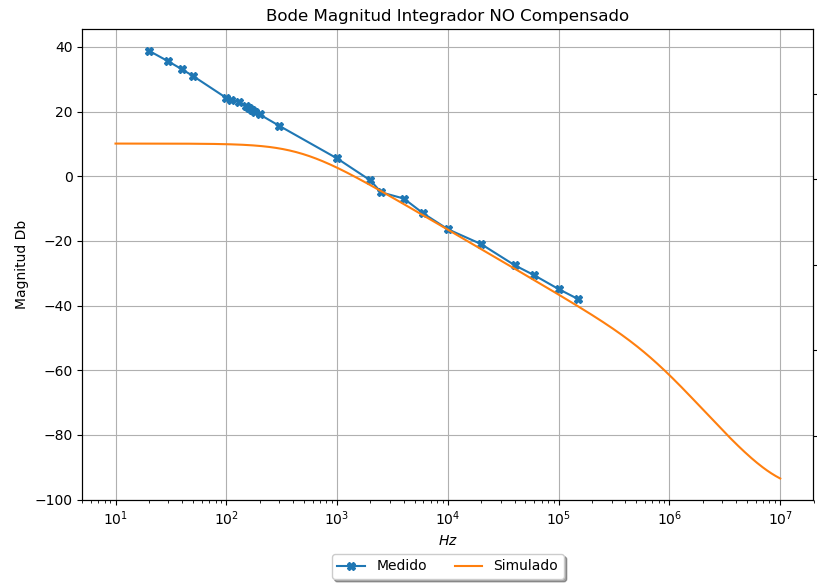
\includegraphics[width=\textwidth]{Ejercicio4/SUPERPOSICION-BODE-INTEGRADOR-NO-COMPENSADO}
	\caption{Bode Integrador NO Compensado}
\end{figure}

%Intentos de medición
\begin{figure}[H]
	\centering
	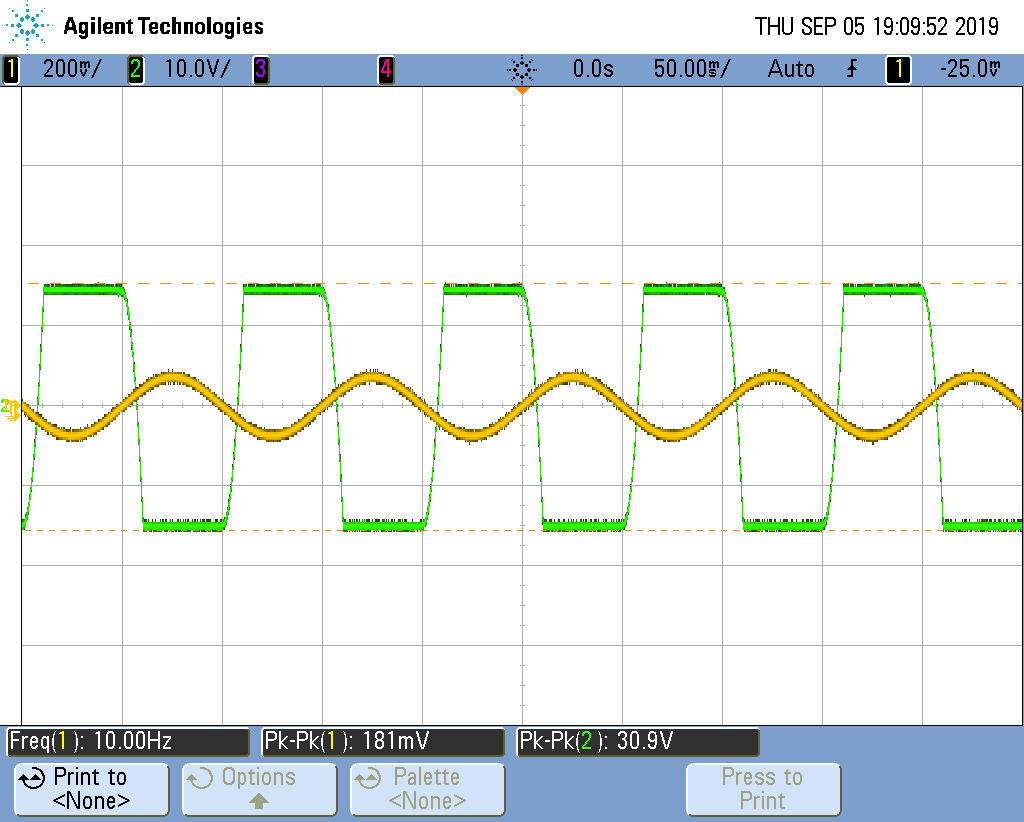
\includegraphics[width=\textwidth]{Ejercicio4/FOTOS-TP2-TC-EJ4/SaturaNoCompensado181mv}
	\caption{Medición a 10Hz 181mVpp}
Se intento reducir la amplitud de la señal de entrada pero los defectos del circuito integrador no permitieron una medición confiable
\end{figure}

\begin{figure}[H]
\centering
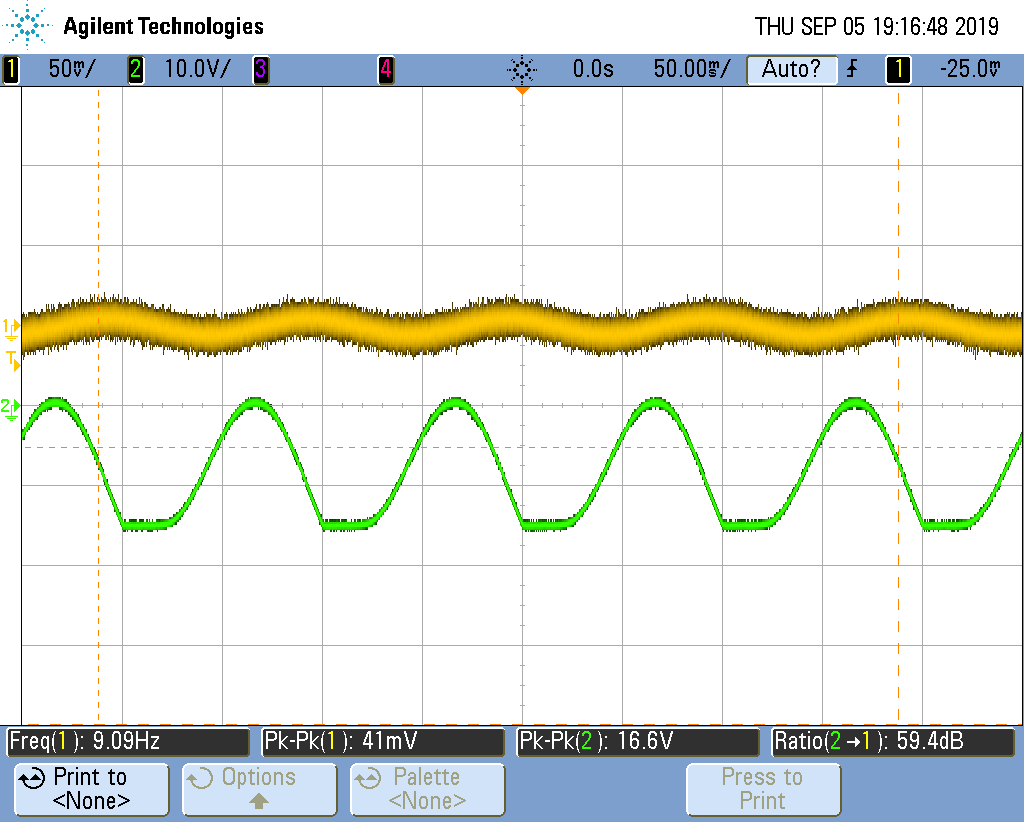
\includegraphics[width=\textwidth]{Ejercicio4/FOTOS-TP2-TC-EJ4/SaturaNoCompensado41}
\caption{Medición a 10Hz 41mVpp}
\end{figure}

Podemos observar que el osciloscopio nos indica una ganancia de 54.4 $dB$. Sin embargo, si vemos con mayor detenimiento la señal de salida tiene su mínimo ubicado en -15V. Lo cual se corresponde con la tensión $V-$ provista a la alimentación del operacional y la cual define el mayor nivel de tensión a la que se puede amplificar.
Este desplazamiento se debe a que el circuito integrador otorga una ganancia muy alta a la componentes de baja frecuencia de la señal. Entre ellas se encuentra la tensión de offset del  propio operacional en adición a las componentes de baja frecuencia de la entrada. Para que ocurra este desplazamiento el circuito integra esa componente constante y no nula. Al integrarlo la señal de baja frecuencia crece como si fuese una rampa hasta llegar a la saturación donde se convierte en una constante. El hecho de que se encuentre en el limito inferior de tensión se debe a la naturaleza inversora del circuito. 
\begin{figure}[H]
	\centering
	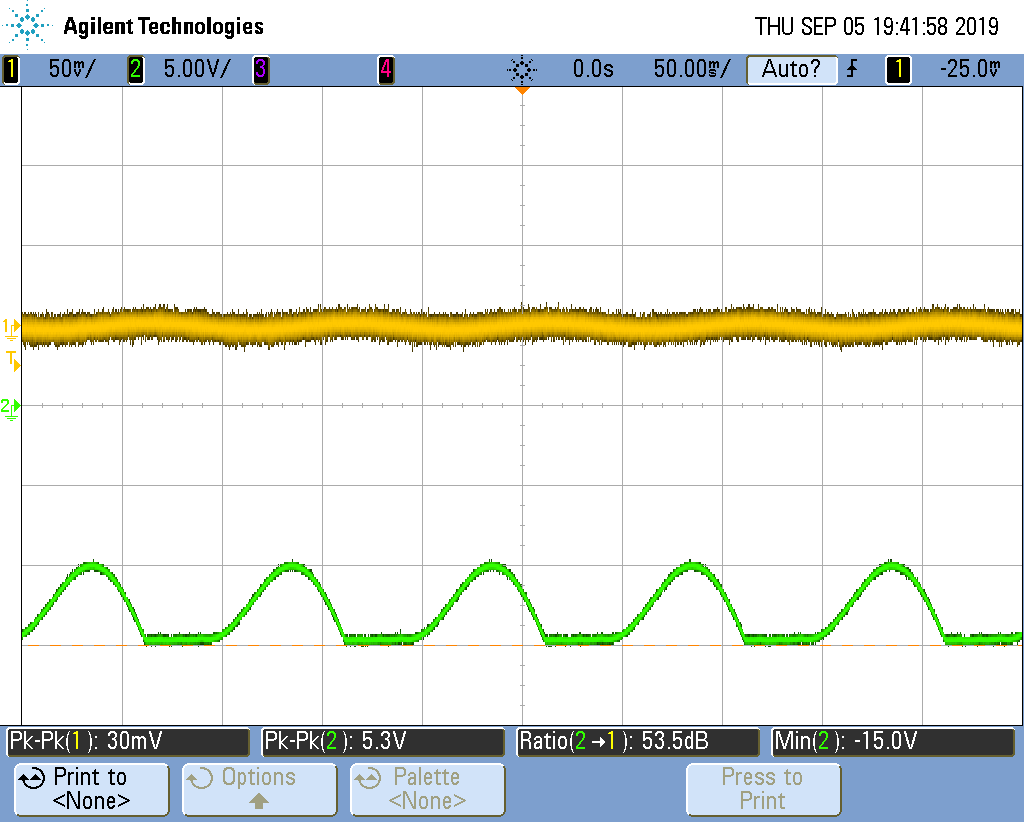
\includegraphics[width=\textwidth]{Ejercicio4/FOTOS-TP2-TC-EJ4/piso}
	\caption{Medición a 10Hz 41mVpp}
\end{figure}

\begin{figure}[H]
	\centering
	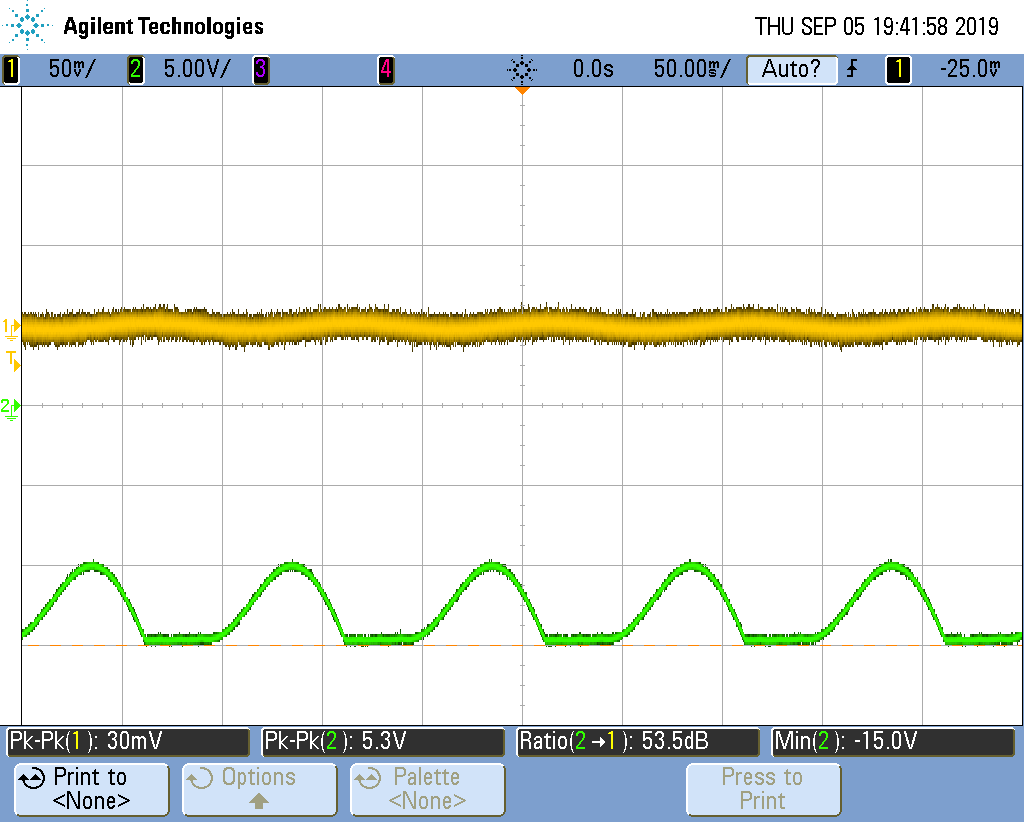
\includegraphics[width=\textwidth]{Ejercicio4/FOTOS-TP2-TC-EJ4/piso}
	\caption{Medición a 10Hz 41mVpp}
\end{figure}

Por las mismas razones de falta de precisión no se presenta el Bode de Fase.
\begin{figure}[H]
	\centering
	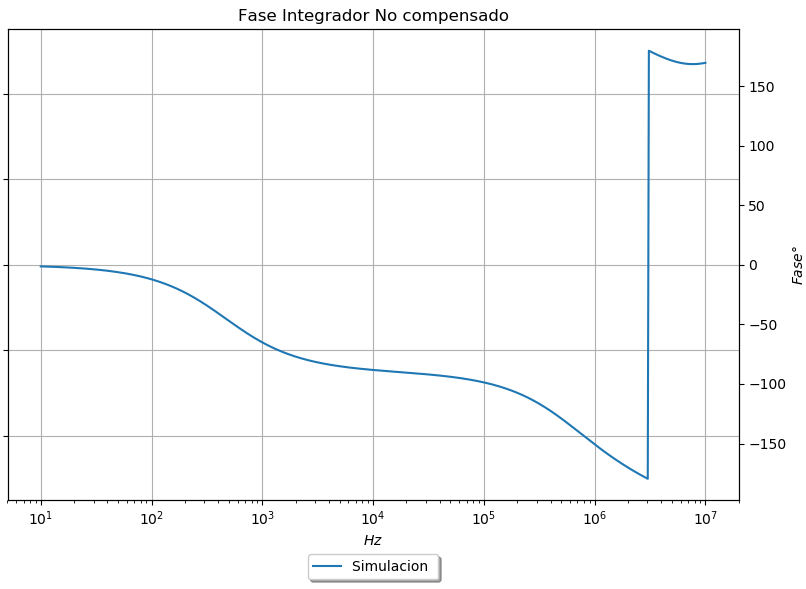
\includegraphics[width=\textwidth]{Ejercicio4/FASE-SIMULADO-INTEGRADOR-NO-COMPENSADO}
	\caption{Medición a 10Hz 41mVpp}
\end{figure}


\subsubsection{Derivador No Compensado}
Se midió la respuesta en frecuencia del derivador sin resistencia de compensación alguna.
\begin{figure}[H]
	\centering
	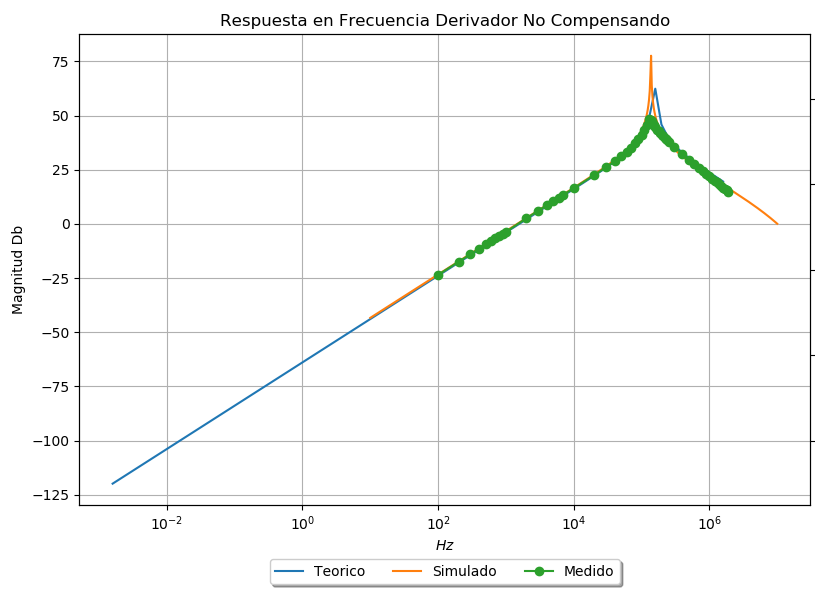
\includegraphics[width=\textwidth]{Ejercicio4/SUPERPOSICION-BODE-DERIVADOR-NO-COMPENSADO}
	\caption{Respuesta en Frecuencia del Circuito Derivador no compensado}
\end{figure}
El circuito derivador, al contrario del integrador, no es capaz de mantener sus capacidades de derivación a lo largo del espectro de frecuencias. Cuando nos aproximamos a frecuencias cercanas a los $140Hz$ el mismo pierde sus propiedades para poder obtener la derivada de la señal de entrada y comienza a comportarse como un integrador. 
El sobre-pico observado es producto de la atenuación causada por el filtro pasabajos que se forma a la entrada del derivador.


\begin{figure}[H]
	\centering
	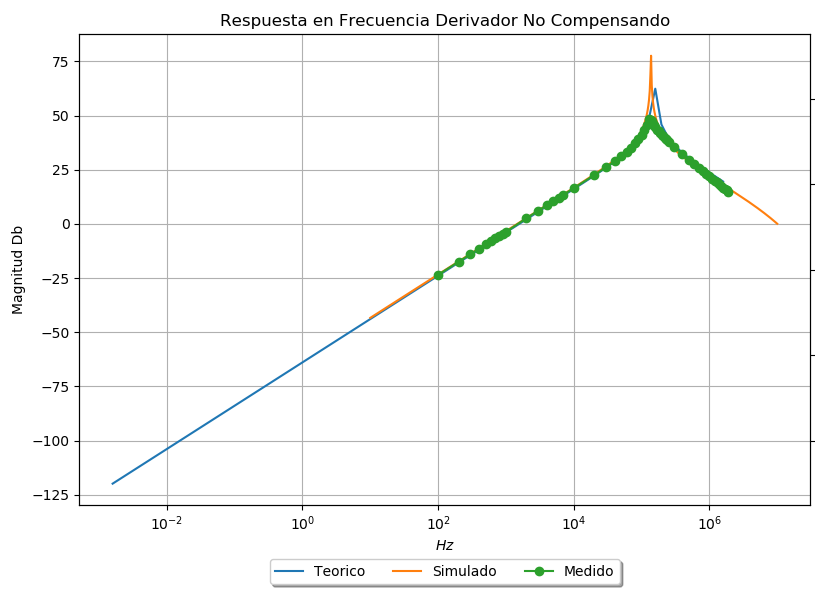
\includegraphics[width=\textwidth]{Ejercicio4/SUPERPOSICION-BODE-DERIVADOR-NO-COMPENSADO}
	\caption{Respuesta en Frecuencia Magnitud del Circuito Derivador no compensado}
\end{figure}

\begin{figure}[H]
	\centering
	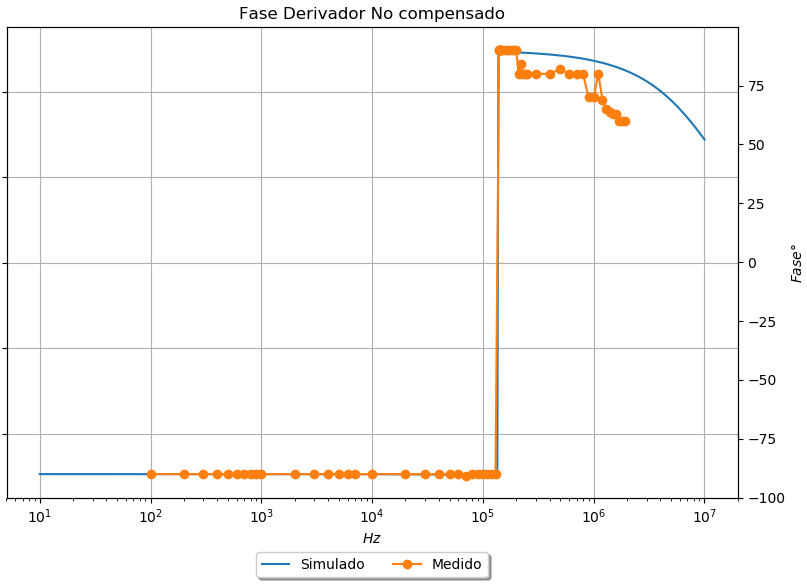
\includegraphics[width=\textwidth]{Ejercicio4/SUPERPOSICION-FASE-DERIVADOR-NO-COMPENSADO}
	\caption{Respuesta en Frecuencia del Fase Circuito Derivador no compensado}
\end{figure}

\section{Respuesta temporal}
En esta sección se exhibirían la respuesta de ambos circuitos bajo diferentes señales de entrada



\begin{figure}[H]
	\centering
	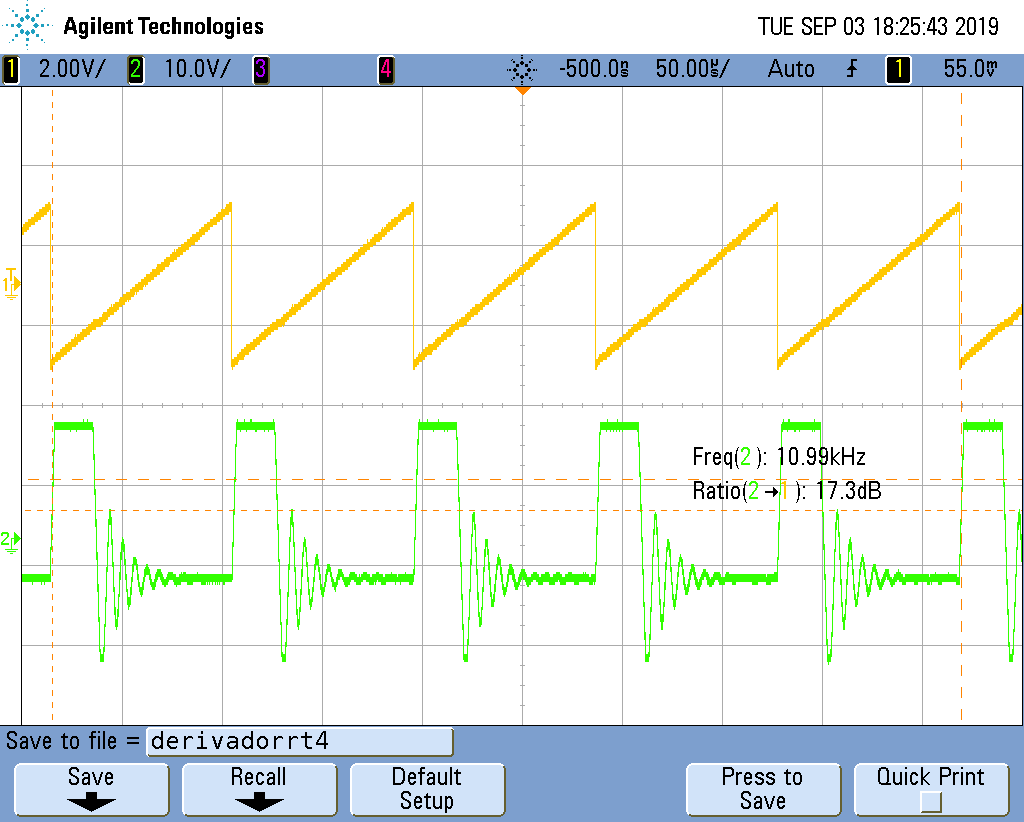
\includegraphics[width=\textwidth]{Ejercicio4/FOTOS-TP2-TC-EJ4/derivadorrt4}
	\caption{Señal dientes de sierra siendo derivada sin compensación}
\end{figure}

\begin{figure}[H]
	\centering
	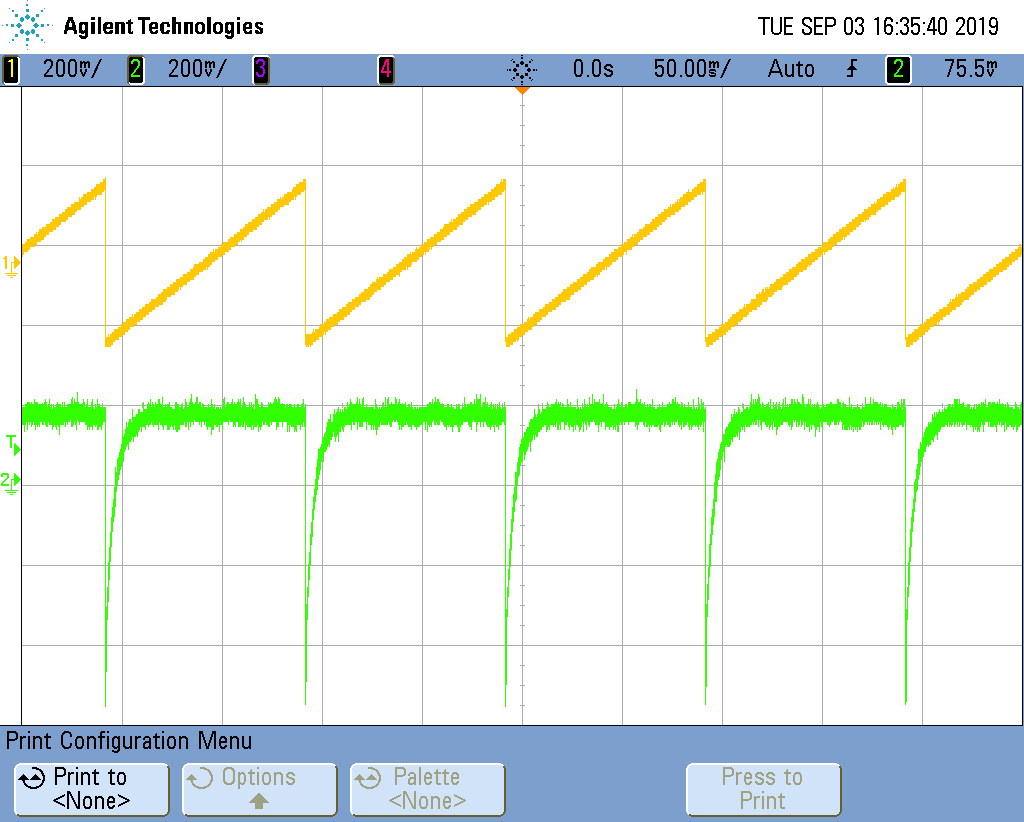
\includegraphics[width=\textwidth]{Ejercicio4/FOTOS-TP2-TC-EJ4/derivador1}
	\caption{Señal dientes de sierra siendo derivada con compensación}
\end{figure}

\begin{figure}[H]
	\centering
	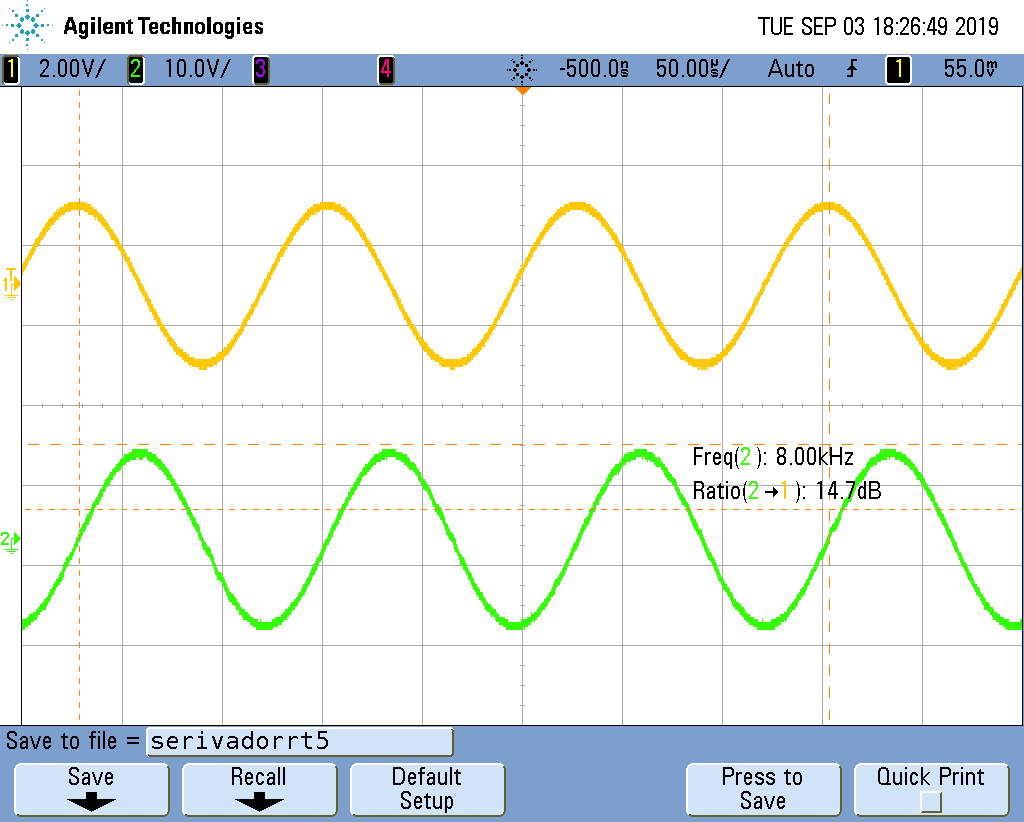
\includegraphics[width=\textwidth]{Ejercicio4/FOTOS-TP2-TC-EJ4/serivadorrt5}
	\caption{Señal Senoidal derivada}
\end{figure}

\begin{figure}[H]
	\centering
	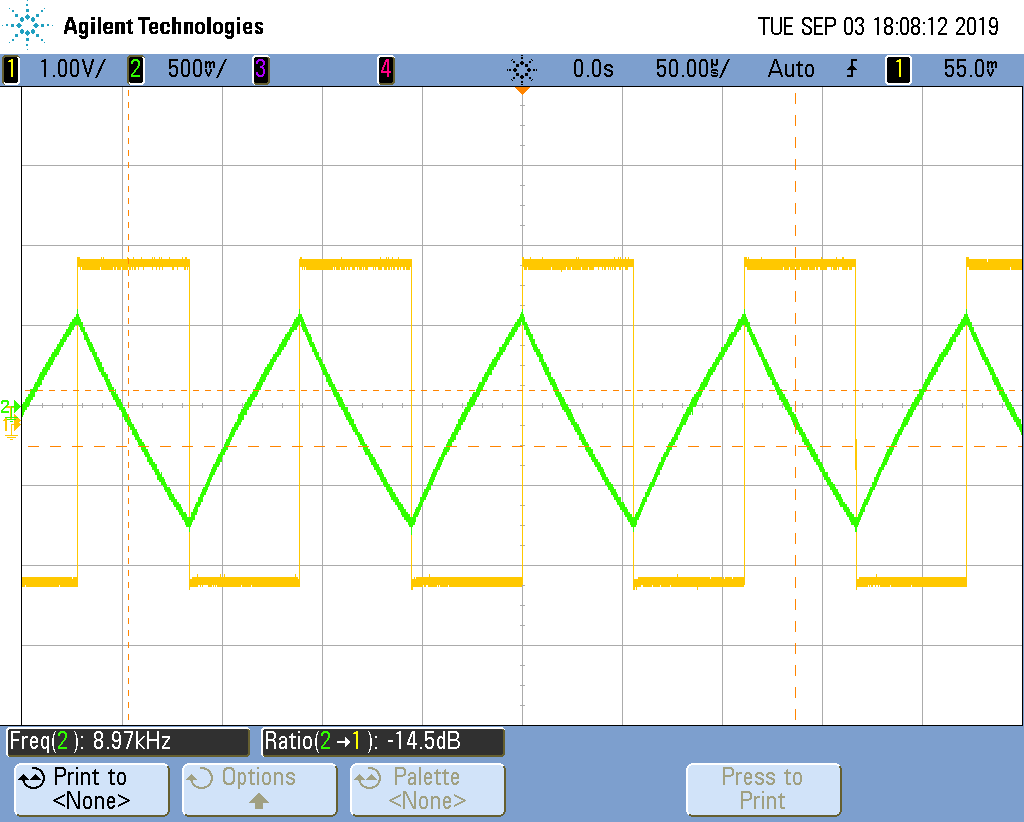
\includegraphics[width=\textwidth]{Ejercicio4/FOTOS-TP2-TC-EJ4/i9tegradort}
	\caption{Onda Cuadrada siendo integrada}
\end{figure}

\begin{figure}[H]
	\centering
	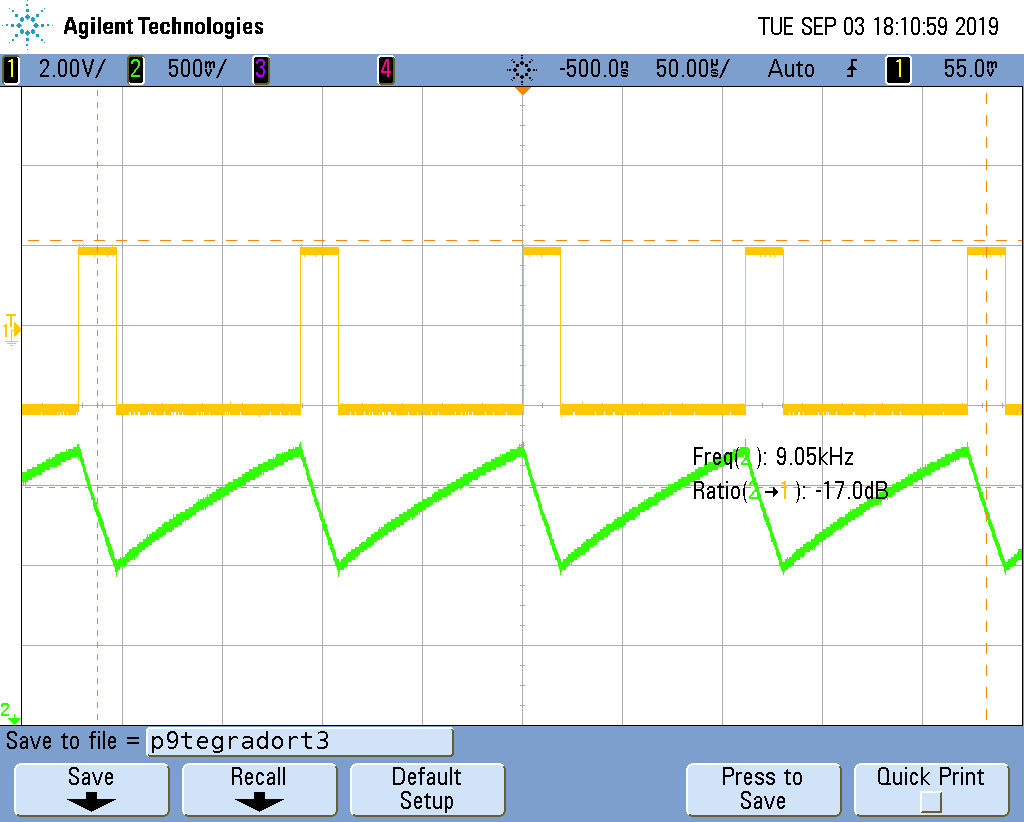
\includegraphics[width=\textwidth]{Ejercicio4/FOTOS-TP2-TC-EJ4/p9tegradort3}
	\caption{Tren de pulsos siendo integrado}
\end{figure}

\begin{figure}[H]
	\centering
	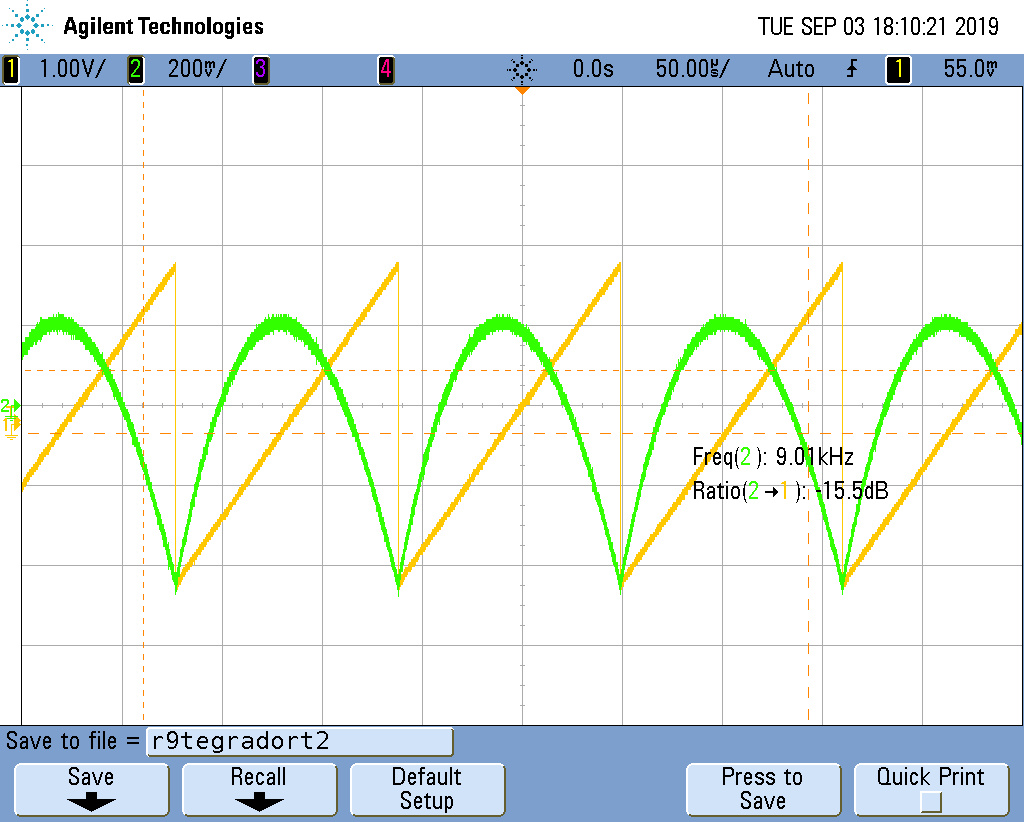
\includegraphics[width=\textwidth]{Ejercicio4/FOTOS-TP2-TC-EJ4/r9tegradort2} 
	\caption{Integral de dientes de sierra}
\end{figure}

\section{Impedancia de Entrada}
Se realizaron las mediciones de impedancia de entrada haciendo uso del analizador de impedancias

\begin{figure}[H]
	\centering
	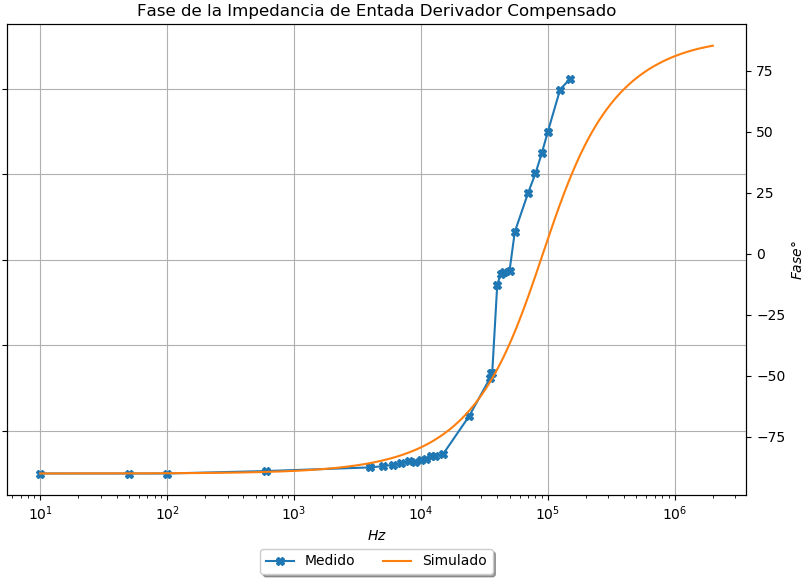
\includegraphics[width=\textwidth]{Ejercicio4/SUPERPOSICION-ZIN-DERIVADOR-COMPENSADO-FASE} 
	\caption{Zin Derivador Compensado}
\end{figure}

\begin{figure}[H]
	\centering
	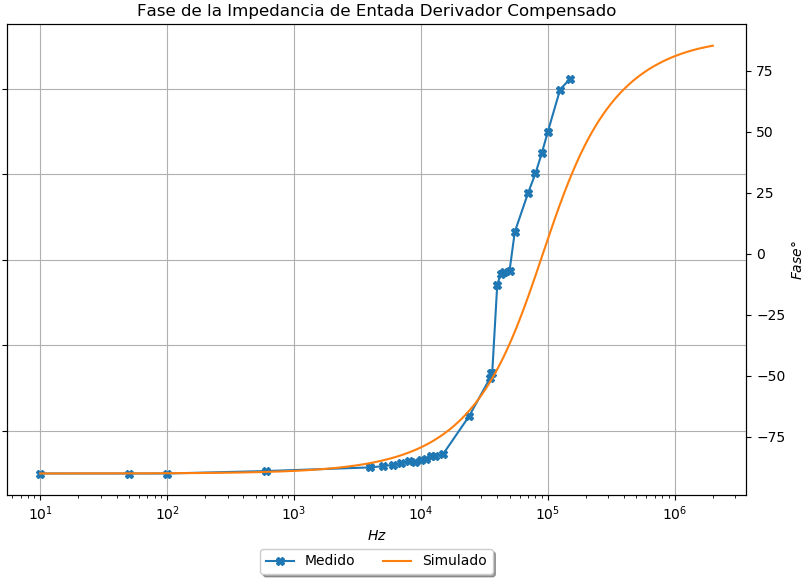
\includegraphics[width=\textwidth]{Ejercicio4/SUPERPOSICION-ZIN-DERIVADOR-COMPENSADO-FASE} 
	\caption{Zin Fase Derivador Compensado}
\end{figure}

\section{Circuitos Compensados}
Como se comento anteriormente, el circuito integrador no operaba de manera optima debido a la tensión de offset que se introducía a la salida a causa de las señales de muy baja frecuencia. Por el otro lado el circuito derivador presenta un sobrepico el cual podría causar daños a un circuito que se conectase a este. 
En el circuito integrador, a bajas frecuencias, su ganancia es muy grande. Es por eso que se debe hacer algo para limitar la ganacias de las mismas. Se podria colocar una resistencia a la entrada pero de ser muy grande arruinaria la transferencia a la salida. Es por eso que se analiza que a bajas frecuencias la impedancia provista por el capacitor es muy grande, comparable con un circuito abierto. Lo cual provocaría que la ganancia del integrador crezca mucho. Por tal motivo se decidió colocar una resistencia en paralelo al capacitor tal que a bajas frecuencias la resistencia limite la ganancia que estas pueden obtener. 
Se decidió colocar una resistencia unas 10 veces más grande de la asignada. 

\begin{figure}[H]
	\centering
	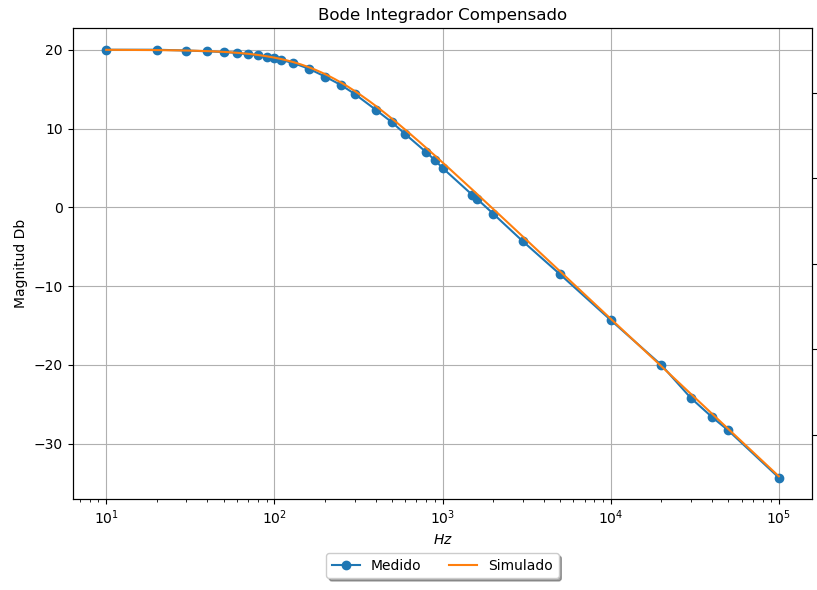
\includegraphics[width=\textwidth]{Ejercicio4/SUPERPOSICION-INTEGRADOR-COMPENSADO} 
	\caption{Bode Magnitud Integrador Compensado}
\end{figure}

\begin{figure}[H]
	\centering
	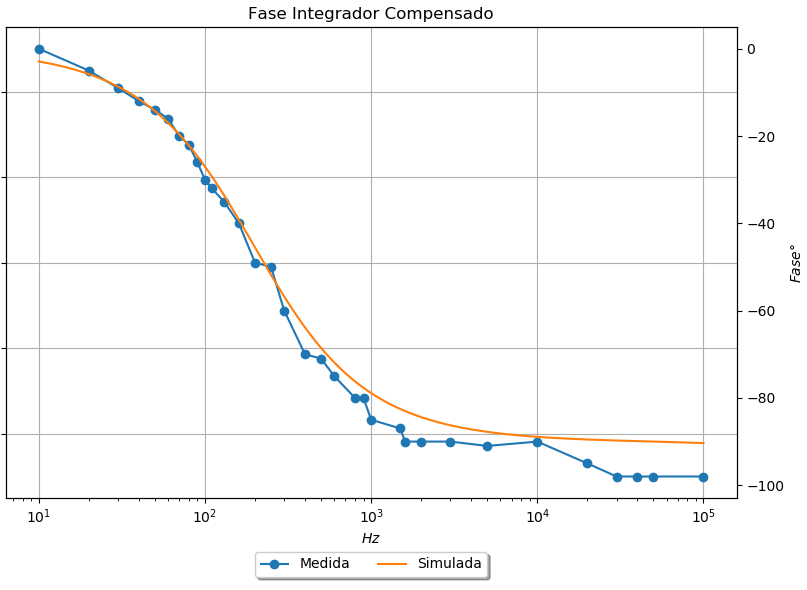
\includegraphics[width=\textwidth]{Ejercicio4/SUPERPOSICION-FASE-INTEGRADOR-COMPENSADO} 
	\caption{Bode Fase Integrador Compensado}
\end{figure}

En el caso del derivador era necesario limitar la ganancia que este podría obtener para así evitar el sobre-pico. A altas frecuencias (aproximadamente $140KHz$ en nuestro caso) el capacitor se comporta como un circuito abierto y se pierde control absoluto sobre la ganacia del circuito al tender esta a infinito. Por lo tanto se coloca una resistencia en serie a la entrada del mismo con el fin de limitar la ganancia.
Se decidió limitar la ganancia a 38$dB$ para poder subsanar el sobre pico. Se escogió una resistencia de 330 $\Omega$.

\begin{figure}[H]
	\centering
	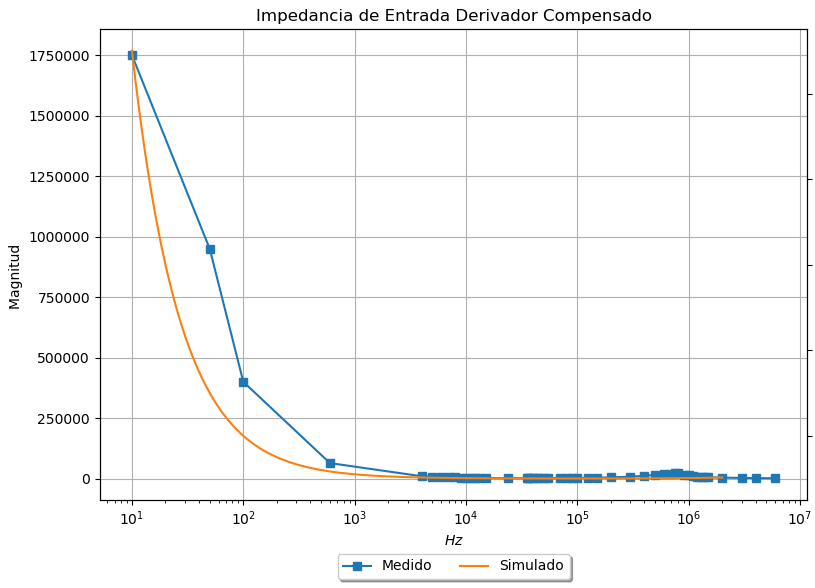
\includegraphics[width=\textwidth]{Ejercicio4/SUPERPOSICION-ZIN-DERIVADOR-COMPENSADO-MAGNITUD} 
	\caption{Bode Magnitud Derivador Compensado}
\end{figure}

\begin{figure}[H]
	\centering
	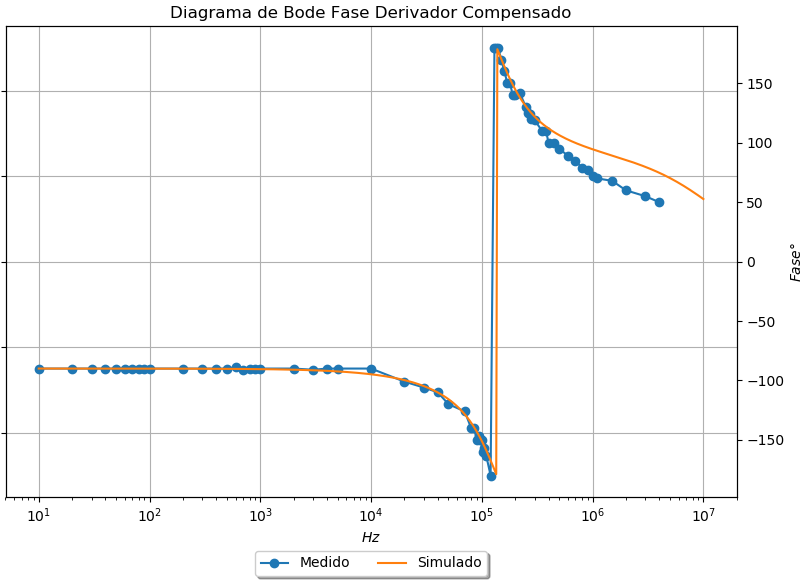
\includegraphics[width=\textwidth]{Ejercicio4/SUPERPOSICION-FASE-DERIVADOR-COMPENSADO} 
	\caption{Bode Fase Derivador Compensado}
\end{figure}

\section{Conclusiones}
Es posible concluir que estos circuitos poseen capacidad de realizar operaciones matemáticas siempre que se encuentren dentro del rango de operación permitido. 
Además se debe tener especial cuidado con las tensiones de off-set del operacional ya que estas pueden influir de manera negativa en el balance de tensiones entre las entradas inversoras y no inversoras. Se pueden estudiar otros métodos de compensación adicional que permitan que los modelos físicos se aproximen lo más a los modelos teóricos. De hecho una mejora que se podría implementar es la de incorporar una resistencia sobre la entrada no inversora que sea de la misma magnitud que la resistencia en serie con la entrada inversora. Esta adición permitirá balancear los voltajes entre sus entradas.   


\end{document}